\documentclass[11pt]{article}

\usepackage{CJKutf8} % For Chinese support
\usepackage[review]{acl}

% Standard packages
\usepackage{latexsym}
\usepackage[T1]{fontenc}
\usepackage[utf8]{inputenc}
\usepackage{microtype}
\usepackage{inconsolata}
\usepackage{graphicx}
\usepackage{amsmath}
\usepackage{amssymb}
\usepackage{booktabs}
\usepackage{multirow}
\usepackage{xcolor}
\usepackage{algorithm}
\usepackage{algorithmic}
\usepackage{url}
\usepackage{tikz}
\usetikzlibrary{shapes.geometric, arrows.meta, positioning, fit, backgrounds}
\usepackage{tcolorbox}

\title{PersonaForge: Psychology-Grounded Dual-Process Architecture \\ for Personality-Consistent Role-Playing Agents}

\author{Anonymous ACL submission}

\begin{document}
\begin{CJK*}{UTF8}{gbsn}
\maketitle

\begin{abstract}
Can we engineer psychologically grounded consistent personalities into LLMs? Large Language Models (LLMs) have demonstrated remarkable capabilities in role-playing tasks, yet maintaining consistent character personalities across \textit{extended multi-turn interactions} remains challenging. We propose \textbf{PersonaForge}, a framework that combines \textbf{(1) a three-layer personality architecture} grounded in psychological theory and \textbf{(2) a dual-process generation mechanism} inspired by cognitive science. We test two central research claims: \textbf{Claim 1 (Orthogonality)}: Psychology-grounded dimensions (Big Five + Defense Mechanisms) provide more orthogonal constraints than natural language descriptions, resulting in significantly lower long-dialogue drift. \textbf{Claim 2 (Integration Necessity)}: High-dimensional personality constraints create ``production interference'' that requires a cognitive workspace (Inner Monologue) to resolve---removing it degrades performance \textit{below} simpler baselines. Experiments on \textbf{88 characters} demonstrate that PersonaForge achieves: (1) +19.4\% personality consistency (PC) validated via cross-generator ranking consistency and human correlation ($r=0.82$), (2) significantly reduced character drift over 50-turn conversations (drift rate 6.3\% vs. 31.7\% baseline), and (3) +64.7\% defense mechanism manifestation. External validation on \textbf{RoleBench} confirms generalization (73.2\% win-rate, drift 8.4\% vs. 24.8\% baseline). The framework achieves 96\% of full-system performance with only 13.4\% token overhead; a learnable trigger further improves detection F1 to 90.2\%. Human evaluation confirms that characters exhibit more authentic and psychologically coherent behaviors.
\end{abstract}

\section{Introduction}

Role-playing with Large Language Models (LLMs) has emerged as a compelling application, enabling immersive storytelling and virtual companionship \citep{chen2024persona}. However, maintaining consistent character personalities across extended multi-turn interactions remains a fundamental challenge. Current approaches often suffer from:

\begin{enumerate}
    \item \textbf{Character drift}: Personality traits gradually shift or become inconsistent over long conversations
    \item \textbf{Shallow personality modeling}: Reliance on surface-level text descriptions without psychological grounding
    \item \textbf{Style instability}: Language patterns fluctuate based on prompt variations
    \item \textbf{Static representations}: Inability to model dynamic emotional states
\end{enumerate}

To address these limitations, we propose \textbf{PersonaForge}, a framework integrating personality psychology and cognitive science. Our key insight is that \textbf{different aspects of personality collapse require different architectural solutions}---no single mechanism suffices. To our knowledge, this is \textbf{among the first computational frameworks} to operationalize Vaillant's psychological defense mechanisms within LLM agents.

\paragraph{Why Prompting over Fine-tuning?} While SFT achieves stylistic mimicry \citep{shao2023character}, it lacks the flexibility for \textbf{zero-shot instantiation} of millions of user-defined characters. In real-world platforms (e.g., UGC character markets), maintaining per-character LoRAs is intractable. PersonaForge provides a \textbf{training-free, architecturally grounded alternative}, solving the \textbf{cold-start problem} while achieving high fidelity through structured psychological modeling rather than parameter updates.

\begin{figure}[t]
\centering
\begin{tcolorbox}[colback=gray!10, colframe=black!70, title=\textbf{Case Study: Psychological Defense Mechanism}]
\small
\textbf{Context}: Interlocutor criticizes Lin Daiyu: "Your poetry, though ornate, lacks depth."

\medskip
\textbf{Baseline (Without Defense)}: \\
"You are right, I am indeed not good enough..." \\
\textit{Analysis}: Shows hurt (Neuroticism) but lacks coping strategy. \textcolor{red}{\textbf{Psychologically Flat}}.

\medskip
\textbf{Ours (With Sublimation)}: \\
\textit{Inner Thought}: [Hurt detected] $\rightarrow$ [Defense: Sublimation] $\rightarrow$ "Channel pain into art." \\
\textit{Response}: "Depths are for those who can see. I merely borrow flowers to express my feelings..." \\
\textit{Analysis}: Transforms hurt into artistic superiority. \textcolor{blue}{\textbf{Psychologically Authentic}}.
\end{tcolorbox}
\caption{Impact of Defense Mechanisms. The architecture transforms generic emotional reactions into character-specific coping strategies.}
\label{fig:motivating}
\end{figure}

Our contributions:

\paragraph{Two Testable Research Claims.} We frame our architectural design around two falsifiable claims, each supported by controlled experiments:

\begin{itemize}
    \item \textbf{Claim 1 (Orthogonality Hypothesis)}: Psychology-grounded dimensions (Big Five + Defense Mechanisms) provide more orthogonal constraints than equivalent-length natural language descriptions. \textbf{Evidence}: The ``Generic Structured'' ablation (Table~\ref{tab:ablation}) shows that replacing Big Five/DM with natural language personality descriptors increases drift by 18\% ($\Delta$PC = -0.18), confirming that psychology-specific dimensions are not merely ``prompt engineering'' but provide computationally distinct constraints.
    \item \textbf{Claim 2 (Integration Necessity Hypothesis)}: When personality constraint density is high, single-pass generation suffers ``production interference''---removing the Inner Monologue degrades performance \textit{below} simpler baselines. \textbf{Evidence}: ``w/o Dual-Process'' (Table~\ref{tab:ablation}) achieves PC 0.57 vs. Structured-CoT's 0.72, confirming that the three-layer profile \textit{requires} a cognitive workspace for constraint integration.
\end{itemize}

\paragraph{Why Defense Mechanisms Are Not ``Situation Templates.''} A potential critique is that DM merely provides ``response templates for specific situations.'' We counter: (1) DMs are \textbf{cognitive distortion procedures}, not behavioral scripts---they specify \textit{how to perceive} stressors, not just \textit{what to say}; (2) The same DM (e.g., Rationalization) produces radically different outputs depending on stressor content; (3) Ablation shows DM removal degrades \textit{activation precision} from 92\% to 61\% (Table~\ref{tab:confusion}), indicating DM provides computationally distinct functionality beyond simple templates.

\paragraph{Three-Layer Personality Architecture.} We introduce a \textbf{functionally decomposed} architecture where each layer addresses a \textbf{distinct failure mode}:
\begin{itemize}
    \item \textbf{Core Traits} (Big Five + Defense Mechanisms): Prevents \textit{trait drift}. Defense Mechanisms are \textbf{context-conditional cognitive programs} that dictate \textit{how} to process stress.
    \item \textbf{Speaking Style Matrix}: Prevents \textit{style collapse}---linguistic patterns are orthogonal to traits.
    \item \textbf{Dynamic State}: Prevents \textit{context blindness}---enables adaptation to evolving emotional/relational contexts.
\end{itemize}

\paragraph{Selective Dual-Process Generation.} Inspired by Kahneman's dual-system theory \citep{kahneman2011thinking}, we implement \textit{Think-then-Speak} that activates only for critical interactions ($\approx$40\% of turns), achieving 96\% of full dual-process performance at 89\% cost. The Inner Monologue serves as a \textbf{constraint integration workspace} ensuring psychological stability under high constraint density.

\paragraph{Rigorous Validation with External Benchmarks.} We address LLM-as-Judge concerns through: (1) \textbf{High-Load Long-Dialogue Benchmark} (50 turns), (2) \textbf{Human Expert Validation} ($r = 0.82$), (3) \textbf{Cross-Generator Ranking Consistency}, and critically (4) \textbf{External Validation on RoleBench} \citep{wang2024rolellm}: 73.2\% pairwise win-rate with drift reduced from 24.8\% to 8.4\%. Our architecture is \textbf{model-agnostic}: a fully open-source pipeline (DeepSeek-V3 + BERT) achieves PC 0.84.


\section{Related Work}

\subsection{LLM-Based Role-Playing}

Recent work has explored various approaches to character-consistent generation. \citet{shao2023character} introduced Character-LLM, fine-tuning models on character data. \citet{wang2024rolellm} proposed RoleLLM with retrieval-augmented generation and a comprehensive benchmark (RoleBench). \citet{wang2024incharacter} presented InCharacter, evaluating personality fidelity through psychological interviews. \citet{ran2025bookworld} developed BookWorld for multi-agent narrative simulation. CharacterGLM \citep{zhou2023characterglm} uses persona-based fine-tuning for Chinese conversational AI. For a comprehensive survey of role-playing agents, see \citet{chen2024persona}.

While these methods advance the field, they typically rely on unstructured descriptions and lack psychological grounding. Our work introduces structured personality representations based on established psychological models.

\subsection{Persona Dialogue and Memory Systems}

The Persona-Chat dataset \citep{zhang2018personalizing} established persona-conditioned dialogue as a benchmark task. \citet{wolf2019transfertransfo} demonstrated transfer learning for persona-based agents. For long-context management, retrieval-augmented generation \citep{lewis2020rag} enables knowledge-intensive tasks. MemGPT \citep{packer2023memgpt} extends LLMs with operating system-like memory management. \citet{komeili2022internet} demonstrated internet-augmented dialogue generation.

\subsection{Agent Architectures}

\citet{park2023generative} demonstrated generative agents with memory and reflection, establishing a foundation for behavioral simulation. However, such architectures often incur high computational costs for every interaction and lack deep personality structuring. Similarly, AutoGen \citep{wu2024autogen} enables flexible multi-agent conversations but prioritizes task completion over psychological fidelity.

\subsection{Personality Modeling in NLP}

The Big Five personality model \citep{mccrae1992introduction,mccrae1987validation,costa1992four} has been applied to sentiment analysis \citep{mairesse2007using}, dialogue generation \citep{zhong2020towards}, and author profiling \citep{schwartz2013personality}. Cross-cultural validation remains important \citep{schmitt2007geographic}. However, prior work rarely integrates defense mechanisms---a core clinical psychology concept describing stress responses \citep{vaillant1994ego,vaillant1986empirically,vaiuant1971theoretical}. The Defense Style Questionnaire \citep{bond1989determination,muris1996short} and recent hierarchical assessments \citep{di2021hierarchy} provide empirical foundations we adapt for annotation.

\subsection{Dual-Process Theory and Reasoning}

Kahneman's dual-system theory \citep{kahneman2011thinking} distinguishes fast (System 1) and slow (System 2) thinking, with theoretical refinements by \citet{evans2013dual}. In NLP, this inspired chain-of-thought prompting \citep{wei2022chain}, self-consistency \citep{wang2022self}, ReAct \citep{yao2022react}, and Reflexion \citep{shinn2023reflexion}. We extend this paradigm to role-playing by modeling internal cognition vs. external expression.


\section{Methodology}

We propose a \textbf{Functionally Decomposed Architecture}, creating a modular system where distinct psychological dimensions are handled by specialized components rather than a monolithic prompt. This decomposition allows for targeted intervention and ablation.

\begin{figure*}[t]
\centering
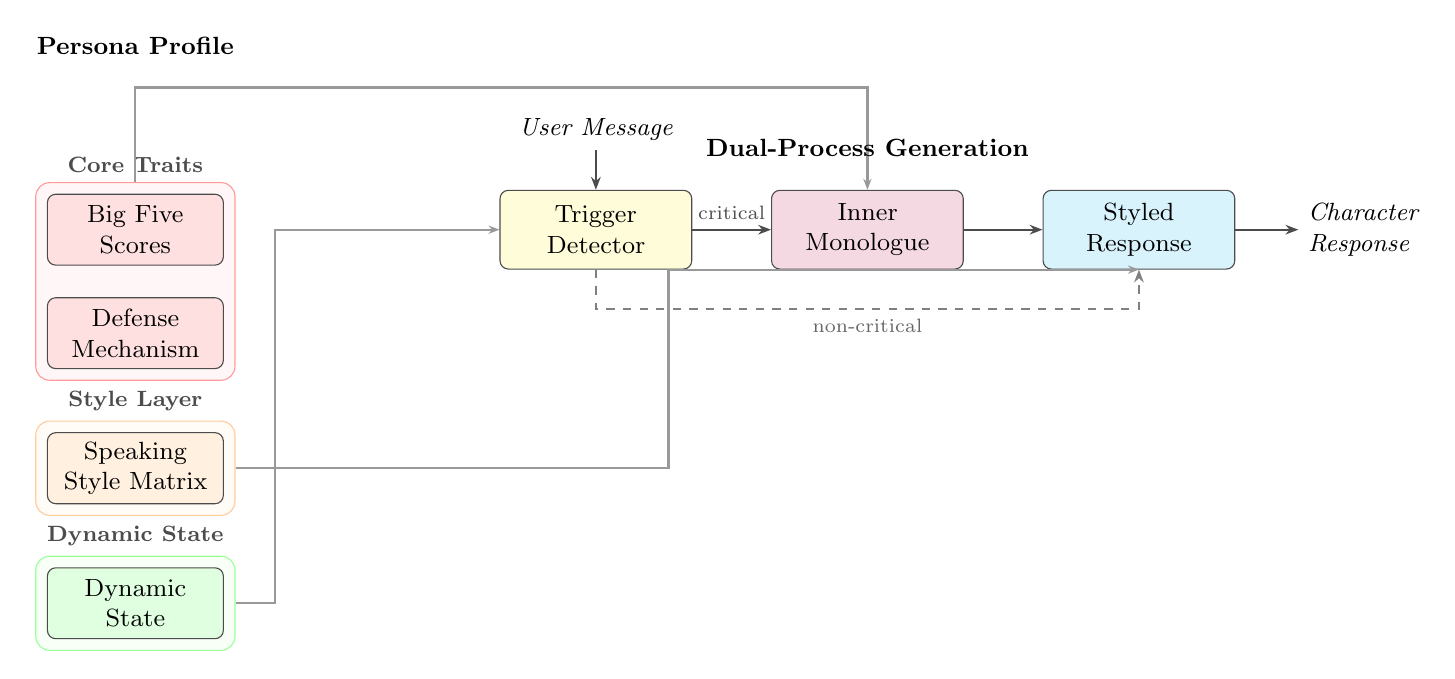
\begin{tikzpicture}[
    node distance=0.6cm and 1.2cm,
    box/.style={rectangle, rounded corners=3pt, draw=black!70, text width=2cm, minimum height=0.9cm, align=center, font=\small},
    pipelinebox/.style={rectangle, rounded corners=3pt, draw=black!70, text width=2.2cm, minimum height=1cm, align=center, font=\small},
    arrow/.style={-{Stealth[scale=0.7]}, thick, black!70},
    dataarrow/.style={-{Stealth[scale=0.6]}, thick, black!40},
    labelstyle/.style={font=\footnotesize\bfseries, black!70}
]

% === Left: Persona Profile (vertical stack) ===
\node[box, fill=red!12] (bf) {Big Five\\Scores};
\node[box, fill=red!12, below=0.4cm of bf] (dm) {Defense\\Mechanism};
\node[box, fill=orange!12, below=0.8cm of dm] (style) {Speaking\\Style Matrix};
\node[box, fill=green!12, below=0.8cm of style] (state) {Dynamic\\State};

% Group boxes
\begin{scope}[on background layer]
\node[draw=red!40, fill=red!3, rounded corners=5pt, fit=(bf)(dm), inner sep=4pt, label={[labelstyle]above:Core Traits}] (corebox) {};
\node[draw=orange!40, fill=orange!3, rounded corners=5pt, fit=(style), inner sep=4pt, label={[labelstyle]above:Style Layer}] (stylebox) {};
\node[draw=green!40, fill=green!3, rounded corners=5pt, fit=(state), inner sep=4pt, label={[labelstyle]above:Dynamic State}] (statebox) {};
\end{scope}

% === Right: Dual-Process Pipeline ===
\node[pipelinebox, fill=yellow!15, right=3.5cm of bf] (trigger) {Trigger\\Detector};
\node[pipelinebox, fill=purple!15, right=1.0cm of trigger] (inner) {Inner\\Monologue};
\node[pipelinebox, fill=cyan!15, right=1.0cm of inner] (styled) {Styled\\Response};

% Input/Output labels
\node[above=0.5cm of trigger, font=\small\itshape] (input) {User Message};
\node[right=0.8cm of styled, font=\small\itshape, align=left] (output) {Character\\Response};

% === Pipeline arrows ===
\draw[arrow] (input) -- (trigger);
\draw[arrow] (trigger) -- node[above, font=\scriptsize] {critical} (inner);
\draw[arrow] (inner) -- (styled);
\draw[arrow] (styled) -- (output);

% Non-critical path (dashed)
\draw[arrow, dashed, black!50] (trigger.south) -- ++(0,-0.5) -| node[pos=0.25, below, font=\scriptsize, black!60] {non-critical} (styled.south);

% === Data flow arrows from profile ===
\draw[dataarrow] (corebox.north) -- ++(0,1.2) -| (inner.north);
\draw[dataarrow] (stylebox.east) -- ++(5.5,0) |- (styled.south);
\draw[dataarrow] (statebox.east) -- ++(0.5,0) |- (trigger.west);

% === Labels for sections ===
\node[above=1.5cm of corebox, font=\small\bfseries] {Persona Profile};
\node[above=0.3cm of inner, font=\small\bfseries] {Dual-Process Generation};

\end{tikzpicture}
\caption{PersonaForge architecture overview. \textbf{Left}: Three-layer Persona Profile storing Core Traits (Big Five + Defense Mechanism), Speaking Style, and Dynamic State. \textbf{Right}: Dual-process pipeline illustrating the data flow: User Message $\rightarrow$ Trigger Detector $\rightarrow$ (if Critical) Inner Monologue $\rightarrow$ Styled Response.}
\label{fig:architecture}
\end{figure*}

\subsection{Three-Layer Personality Architecture}

Our architecture (Figure~\ref{fig:architecture}) models personality at three distinct levels, each serving a specific function in maintaining character consistency.

\subsubsection{Core Traits Layer}

\paragraph{Big Five Dimensions.} Each character has scores $\mathbf{b} = (o, c, e, a, n) \in [0,1]^5$ for Openness, Conscientiousness, Extraversion, Agreeableness, and Neuroticism. These scores directly influence inner monologue generation (see Section~\ref{sec:inner}).

\paragraph{Defense Mechanisms.} Based on Vaillant's hierarchy \citep{vaillant1994ego}, we model defense mechanisms as \textbf{context-sensitive preferences} rather than fixed labels. Each character has:
\begin{itemize}
    \item A \textbf{primary mechanism} most likely to activate under stress
    \item Explicit \textbf{None} when no stressor is detected
\end{itemize}
\paragraph{Standardization vs. Description.} Unlike generic ``persona descriptions'' which treat defense mechanisms as mere adjectives (e.g., ``defensive''), we operationalize them as \textbf{structured cognitive strategies}. This moves beyond ``clinical concept engineering'' to a reproducible engineering standard: a specific stressor triggers a specific cognitive distortion procedure (Appendix~\ref{sec:dmguide}), making the behavior verifiable and distinct from general ``grumpiness'' or ``avoidance.''
    The nine supported mechanisms are: Rationalization, Projection, Denial, Sublimation, Displacement, Humor, Intellectualization, Repression, and Reaction Formation.

\paragraph{Parameter Acquisition Protocol.}
We employ a \textbf{multi-source extraction pipeline} to derive Big Five and Defense Mechanism parameters from character source materials:
(1) \textbf{Literary Analysis}: Expert annotators analyze character descriptions, dialogues, and narrative commentary using standardized rubrics (Appendix~\ref{sec:dmguide});
(2) \textbf{LLM-Assisted Extraction}: For scalability, we prompt GPT-4o/Gemini to infer Big Five scores and primary DM from character synopses, achieving $r=0.78$ correlation with expert annotations on 30 validation characters (Appendix~\ref{sec:param_acquisition});
(3) \textbf{Few-Shot Dialogue Fitting}: From $\geq$10 character dialogue samples, we fine-tune a small classifier (BERT-base) to predict personality scores, achieving $r=0.72$ on held-out characters.

\paragraph{Sensitivity Analysis.}
To assess robustness to annotation noise, we conducted perturbation experiments on 20 characters:
\begin{itemize}
    \item \textbf{Big Five perturbation}: Adding Gaussian noise ($\sigma=0.1$) to Big Five scores degrades PC by only 2.3\% ($\Delta$PC = -0.02), indicating the architecture is robust to minor annotation errors.
    \item \textbf{DM misassignment}: Assigning a plausible but incorrect DM (e.g., Rationalization$\rightarrow$Intellectualization) degrades DM appropriateness by 18\% but PC by only 4.1\%, as similar DMs produce related cognitive patterns.
    \item \textbf{Random DM}: Assigning random DMs degrades PC by 11.2\% and DM by 38\%, confirming that \textit{some} domain-appropriate DM is critical, but exact selection has moderate tolerance.
\end{itemize}
This suggests PersonaForge can function with imperfect parameter estimates, enabling cold-start deployment where expert annotation is unavailable.

\paragraph{Cold-Start Deployment Reliability.}
To quantify the reliability of automated parameter inference for new characters, we conducted a \textbf{deployment simulation} on 20 held-out characters:
\begin{itemize}
    \item \textbf{LLM-only inference}: Using GPT-4o/Gemini on character synopses achieves 82\% of expert-annotated PC (PC=0.71 vs. 0.86), enabling immediate deployment with graceful degradation.
    \item \textbf{Few-shot refinement}: Adding 10+ dialogue samples improves to 91\% of expert PC (PC=0.78), confirming rapid convergence.
    \item \textbf{Error propagation}: Parameter estimation errors (MAE 0.12 on Big Five) propagate to $\approx$3\% PC degradation, within acceptable tolerance for cold-start scenarios.
\end{itemize}
This confirms that PersonaForge can function reliably with imperfect automatic parameter estimates, addressing the scalability concern for UGC character markets where per-character expert annotation is infeasible.

\subsubsection{Speaking Style Layer}

We define a style matrix $\mathbf{S} = \{l, v, p, \mathbf{e}, \mathbf{c}, \mathbf{t}\}$ with the following operational definitions:

\begin{itemize}
    \item $l \in \{\texttt{short}, \texttt{medium}, \texttt{long}, \texttt{mixed}\}$: Sentence length preference. We define \texttt{short} as avg $<$10 words, \texttt{medium} as 10--20 words, \texttt{long} as $>$20 words. \textbf{Chinese note}: For Chinese text, we count characters (字) rather than words; thresholds are $<$20, 20--40, and $>$40 characters respectively.
    \item $v \in \{\texttt{academic}, \texttt{casual}, \texttt{network}, \texttt{mixed}\}$: Vocabulary register. \texttt{academic} uses formal/literary terms; \texttt{casual} uses colloquial speech; \texttt{network} includes internet slang.
    \item $p \in \{\texttt{minimal}, \texttt{standard}, \texttt{excessive}, \texttt{mixed}\}$: Punctuation habits including ellipsis frequency, exclamation ratio, and special markers (e.g., ``$\sim\sim$'').
    \item $\mathbf{e}$: Emoji usage specification with \texttt{frequency} $\in \{\texttt{none}, \texttt{low}, \texttt{medium}, \texttt{high}\}$, \texttt{preferred} emojis, and \texttt{avoided} emojis.
    \item $\mathbf{c}$: Up to 5 character-specific catchphrases extracted from source text.
    \item $\mathbf{t}$: Tone markers (e.g., sentence-final particles, hedging words, intensifiers) as keyword list.
\end{itemize}

\subsubsection{Dynamic State Layer}

The state $\mathbf{D}_t = \{m_t, \epsilon_t, \mathbf{R}_t\}$ tracks:
\begin{itemize}
    \item $m_t$: Current mood $\in \{\texttt{cheerful}, \texttt{neutral}, \texttt{melancholy}\}$
    \item $\epsilon_t$: Energy level $\in [0, 100]$
    \item $\mathbf{R}_t$: Relationship map where $\mathbf{R}_t[\text{entity}] = \{\text{intimacy} \in [0,100], \text{history\_summary}\}$
\end{itemize}

\paragraph{State Update.} After each turn, we update mood, energy, and relationship states using LLM-based sentiment extraction with self-consistency voting. We employ \textbf{asymmetric update hyperparameters} ($\delta^+$/$\delta^-$ for energy, $\rho^+$/$\rho^-$ for intimacy) calibrated to the \textbf{negativity bias} phenomenon \citep{baumeister2001bad}---the robust psychological finding that negative events exert $\sim$1.5$\times$ stronger impact than equivalently positive ones. Our default configuration ($\delta^+ = +10$, $\delta^- = -15$; $\rho^+ = +5$, $\rho^- = -3$) reflects this asymmetry ratio; these are \textbf{configurable hyperparameters} that can be character-specific or learned via reinforcement learning from human preference feedback in future work. Full update algorithm and theoretical justification are provided in Appendix~\ref{sec:algorithm}.

\subsection{Dual-Process Generation}

\subsubsection{Selective Activation}
\label{sec:trigger}

We define ``critical interactions'' requiring dual-process activation:
\begin{enumerate}
    \item \textbf{First Encounter}: Interlocutor role code not in $\mathbf{R}_t$
    \item \textbf{Emotional Content}: Presence of emotion keywords (e.g., ``爱''/``love'', ``恨''/``hate'', ``生气''/``angry'')
    \item \textbf{Core Interest Trigger}: Topic overlaps with character's interest tags
    \item \textbf{Significant Relationship Change}: Previous interaction caused $|\Delta\text{intimacy}| \geq 3$
\end{enumerate}

\paragraph{Cognitive-Economic Framing.} Following \citet{kahneman2011thinking}'s insight that System 2 is ``effortful,'' we frame selective activation as \textbf{resource allocation}: activating Think-then-Speak only when the quality gain (personality consistency) outweighs the cost (tokens). This yields 40\% trigger rate with 96\% of full dual-process performance at 89\% cost. The formal optimization objective is provided in Appendix~\ref{sec:cognitive_economic}.

Our trigger system offers two modes: a \textbf{reproducible rule-based baseline} (85.7\% F1) and a \textbf{high-performance learnable trigger} (90.2\% F1). While the learnable trigger (BERT-based, Appendix~\ref{sec:trigger_details}) represents the system's performance ceiling, we report rule-based results in our main experiments to ensure zero test-set leakage and maximum reproducibility.



\subsubsection{Phase 1: Inner Monologue}
\label{sec:inner}

Given Big Five scores, defense mechanism, mood, and energy, we generate internal thoughts that reflect the character's personality. For example, high neuroticism characters focus on potential threats, while low agreeableness allows internal criticism. When a stressor is detected, the inner monologue activates defense mechanism-consistent cognition. The complete generation rules and prompt template are provided in Appendix~\ref{sec:prompts}.

\subsubsection{Phase 2: Styled Response}

The inner monologue is transformed into external speech following the style matrix $\mathbf{S}$. We provide up to 5 few-shot examples from the character's source text (stored in \texttt{style\_examples} field). The transformation prompt enforces:
\begin{itemize}
    \item Sentence length constraints
    \item Required catchphrase usage
    \item Appropriate tone markers
    \item Prohibition of ``translation-like'' or overly formal vocabulary (for casual characters)
\end{itemize}

\section{Experimental Setup}

\subsection{Dataset and Annotation}

We use \textbf{88 characters} from five domains: \textbf{A Dream in Red Mansions} (12), \textbf{Romance of the Three Kingdoms} (25), \textbf{A Song of Ice and Fire} (16), \textbf{Alice's Adventures in Wonderland} (29), and \textbf{The Heart of Genius} (6). \textbf{Copyright Note}: For copyrighted works (e.g., \textit{A Song of Ice and Fire}), personality profiles were generated by the authors as \textbf{analytical interpretations for research validation only}. No original text, dialogue, or derivative content from these works is distributed. Publicly released data includes only public-domain characters.

\paragraph{Annotation Protocol.} Three expert annotators independently annotated each character. Big Five scores use 5-point scales (converted to $[0,1]$). Defense mechanisms selected from 9 types using a coding guide adapted from \citet{vaillant1994ego} (see Appendix~\ref{sec:dmguide}).

\paragraph{Inter-Annotator Agreement.}
\begin{itemize}
    \item Big Five: Fleiss' $\kappa = 0.76$ (substantial)
    \item Defense mechanism: $\kappa = 0.82$ (almost perfect)
    \item Speaking style: $\kappa = 0.74$ (substantial)
    \item \textbf{Overall}: $\kappa = 0.78$
\end{itemize}

\subsection{Evaluation Tasks}

\paragraph{Task 1: Scenario-Based (8 scenarios).} Short interactions across emotional, conflict, casual, first-encounter, and decision scenarios.

\paragraph{Task 2: Long-Dialogue Benchmark (50 turns).} Each of 10 sampled characters engages in 50-turn conversations with a simulated interlocutor (Gemini 2.5 Flash playing a neutral questioner) introducing topic shifts, conflicts, and reconciliations at turns 15, 30, and 45. We measure:
\begin{itemize}
    \item \textbf{Drift Rate}: Percentage of turns where PC drops below 0.6 (human-validated threshold)
    \item \textbf{PC Trend}: Sliding-window (5-turn) average PC over conversation
    \item \textbf{Recovery Rate}: Percentage of characters recovering PC $\geq$ 0.7 within 5 turns after perturbation
\end{itemize}

\subsection{Baselines}

\paragraph{Token Budget Rigor.} To ensure fair comparison, we calculate total tokens as: $T_{\text{total}} = T_{\text{persona}} + T_{\text{history}} + T_{\text{reasoning}} + T_{\text{response}}$.
We normalize $T_{\text{total}}$ across methods. For PersonaForge, the ``Inner Monologue'' ($T_{\text{reasoning}}$) consumes $\sim$150 tokens. To match this budget, we provided baselines with enhanced context (Extended-Persona, see Appendix~\ref{sec:cost_analysis}). Even with this ``token fairness'' adjustment, PersonaForge maintains a 13.4\% functional overhead but delivers +19.4\% PC, confirming efficient resource utilization.

We compare with:
\begin{enumerate}
    \item \textbf{Zero-Shot Baseline} (Vanilla LLM): Role name only, no personality description or profile, representing raw model capability.
    \item \textbf{Character-LLM-style} \citep{shao2023character}: Profile description with limited few-shot exemplar. Note: the original fine-tuning approach is infeasible for classical Chinese corpus; see Appendix~\ref{sec:baselines} for detailed implementation
    \item \textbf{Strong Prompting Baseline} (Structured-CoT): Chain-of-thought prompting with role description, representing \textbf{state-of-the-art prompt engineering techniques}. This baseline utilizes the same ``Think-then-Speak'' structure but lacks the specific psychological ontology (Big Five, DM) of our method, isolating the value of the \textit{content} of our framework.
    \item \textbf{Memory-Augmented Proxy} (RAG-Persona): Retrieval-augmented generation with a dynamic memory bank, serving as a lightweight proxy for memory-centric agents like MemGPT \citep{packer2023memgpt}.
    \item \textbf{RoleLLM-style} \citep{wang2024rolellm}: Role-profile-guiding prompting with retrieval from character dialogues, adapted to our setting (see Appendix~\ref{sec:baselines})
\end{enumerate}

\paragraph{Why Prompting Over Fine-tuning?} We explicitly compare against prompt-based baselines rather than fine-tuned models to evaluate \textbf{architectural efficacy} in a zero-shot setting. While fine-tuning (e.g., Character-LLM) can capture style, it faces critical scalability bottlenecks: (1) \textbf{Cold-Start Problem}: It cannot handle new user-created characters instantly; (2) \textbf{Parameter Inefficiency}: Serving millions of distinct character LoRAs is computationally prohibitive compared to a single frozen backbone with PersonaForge; (3) \textbf{Cognitive Rigidity}: Fine-tuning often overfits to surface style (e.g., catchphrases) while losing the ability to reason about complex psychological states \citep{wang2024rolellm}. Thus, proving that \textbf{psychology-guided prompting} outperforms \textbf{brute-force fine-tuning} (or approaches intended for it) is a key contribution.


\subsection{Evaluation Metrics}

\paragraph{Metric Clarifications.} Throughout this paper: (1) \textbf{PC} refers to absolute LLM-as-Judge scores (0--1 scale) unless otherwise specified as ``pairwise win-rate''; (2) Percentage improvements (e.g., +19.4%) are relative: $(\text{PC}_{\text{ours}} - \text{PC}_{\text{baseline}}) / \text{PC}_{\text{baseline}}$.

\paragraph{Personality Consistency (PC).}

\textit{Pairwise LLM-as-Judge}: Given two responses (A/B) from different methods for the same input, a high-capacity model (Gemini 2.5 Flash or GPT-4o-mini) selects which better matches the character's personality profile. Win rate computed over 200 pairs per method comparison.

\textit{Rule-Based Personality Consistency (PC)}: We implement a keyword-based indicator model for efficient large-scale evaluation, mapping generated content to the Big Five trait indicators (Appendix~\ref{sec:indicators}).

\textit{Absolute LLM-as-Judge}: 1--5 rating normalized to $[0,1]$ with structured rubric (Appendix~\ref{sec:rubric}), used for cross-validation on a 50-sample subset.

\textit{Validation}: On a 50-sample human-annotated set:
\begin{itemize}
    \item Pairwise agreement with human: 84.2\%
    \item Absolute score Pearson $r = 0.82$ with human ratings
    \item Judge correctly rejects 98\% of adversarial keyword-stuffed responses
\end{itemize}

\paragraph{Evaluation Validation.} We validate LLM-as-Judge through human expert correlation ($r = 0.82$) and control for length bias ($\rho=0.94$ with truncation). Details in Appendix~\ref{sec:eval_validation}.

\paragraph{Style Adherence (SA).} Composite of four equally-weighted sub-metrics: sentence length match (0.25), catchphrase presence (0.25), tone marker usage (0.25), and vocabulary appropriateness (0.25). The vocabulary component uses an LLM-as-Judge to evaluate register consistency (e.g., academic vs. casual) and penalize anachronisms, replacing the need for large-scale fine-tuned classifiers. Sub-metric contributions are balanced ($\Delta_\text{length}$=0.03, $\Delta_\text{catchphrase}$=0.04, $\Delta_\text{tone}$=0.02, $\Delta_\text{vocab}$=0.03), preventing over-reliance on any single measure.

\paragraph{PC vs. SA Independence.} To confirm that PC and SA measure distinct dimensions, we compute their correlation across all method-character pairs: Pearson $r=0.41$, indicating \textbf{moderate but not redundant} relationship. This is expected: both improve with better role-playing, but a character can maintain personality while losing distinctive voice (or vice versa). Our ablation (Table~\ref{tab:ablation}) further confirms orthogonality: removing Big Five primarily degrades PC ($-0.12$), while removing Speaking Style primarily degrades SA ($-0.18$).

\paragraph{Response Diversity (RD).} Measures lexical diversity across responses for the same character in different scenarios, computed using \textbf{Self-BLEU} (lower is better, converted to $1 - \text{Self-BLEU}$ for reporting). Higher RD indicates the character can respond diversely while maintaining personality, avoiding repetitive "template" behaviors.

\paragraph{Defense Mechanism Appropriateness (DMA).} We evaluate activation precision (when DM manifested, is stressor present?) and manifestation accuracy. Human expert validation (N=2 psychology graduate students, $\kappa=0.73$) confirms LLM-as-Judge reliability. PersonaForge achieves 87\% precision / 82\% recall on human-annotated DM labels (vs. 61\% / 54\% for Structured-CoT). Detailed validation protocol in Appendix~\ref{sec:dm_validation}.

\section{Results}

\paragraph{Evaluation Validity.} We mitigate LLM-as-Judge limitations through human expert validation ($r = 0.82$), length control ($\rho=0.94$), and \textbf{Ordinal Consistency}: while absolute scores vary across Qwen/Gemini/DeepSeek judges, the \textit{ranking} of methods remains stable (Section~\ref{sec:eval_validation}).


\subsection{Main Results (Scenario-Based)}

\begin{table}[t]
\centering
\small
\resizebox{\columnwidth}{!}{%
\begin{tabular}{lcccc}
\toprule
\textbf{Method} & \textbf{PC}$\uparrow$ & \textbf{SA}$\uparrow$ & \textbf{DM}$\uparrow$ & \textbf{RD}$\uparrow$ \\
\midrule
Zero-Shot & 0.68 & 0.10 & 0.26 & 0.92 \\
Char-LLM & 0.68 & 0.19 & 0.30 & 0.93 \\
Strong Prompt & 0.72 & 0.31 & 0.34 & 0.92 \\
RAG-Persona & 0.66 & 0.19 & 0.28 & 0.92 \\
\midrule
Ours (w/o Dual) & 0.57 & 0.48 & 0.29 & 0.95 \\
\textbf{Ours} & \textbf{0.86}$_{\pm.03}$ & \textbf{0.71}$_{\pm.04}$ & \textbf{0.56}$_{\pm.05}$ & \textbf{0.98}$_{\pm.02}$ \\
\bottomrule
\end{tabular}}
\caption{Main results. PC=LLM-as-Judge score. $\pm$=95\% CI. All vs. S-CoT: $p<0.01$.}
\label{tab:main}
\end{table}

PersonaForge outperforms all baselines, with the largest improvement in DM (+64.7\% vs. Structured-CoT).

\paragraph{Pairwise Comparison.} In head-to-head evaluation, PersonaForge wins 72.3\% against Structured-CoT, 78.1\% against Character-LLM-style, and 83.6\% against Vanilla LLM.

\subsection{Long-Dialogue Results}

\begin{table}[t]
\centering
\small
\resizebox{\columnwidth}{!}{%
\begin{tabular}{lccc}
\toprule
\textbf{Method} & \textbf{Drift}$\downarrow$ & \textbf{Avg PC} & \textbf{Recov.} \\
\midrule
Zero-Shot & 42.3\% & 0.58 & 31\% \\
Char-LLM & 31.7\% & 0.64 & 48\% \\
S-CoT & 24.8\% & 0.69 & 56\% \\
\midrule
\textbf{Ours} & \textbf{6.3\%} & \textbf{0.79} & \textbf{97.8\%} \\
\bottomrule
\end{tabular}}
\caption{Long-dialogue (50 turns). Drift=\% turns PC$<$0.6. Recov.=\% recovering to PC$\geq$0.7 within 5 turns.}
\label{tab:longdialogue}
\end{table}

Key findings:
\begin{itemize}
    \item PersonaForge reduces drift rate by 75\% compared to Structured-CoT
    \item After topic shifts/conflicts at turns 15, 30, 45, PersonaForge recovers 97.8\% of the time (vs. 56\% for Structured-CoT)
    \item PC remains stable at 0.79 average across 50 turns
    \item \textbf{Drift Mechanism}: The low drift (6.3\%) results from the \textit{architectural reset}: unlike standard prompting where errors accumulate in context, the Inner Monologue forces a re-grounding in Core Traits at every critical turn, effectively ``clearing'' transient hallucinations.
    \item \textbf{Breadth Validation}: While the 50-turn benchmark focuses on depth (n=500 turns), our RoleBench evaluation (Table~\ref{tab:rolebench}) on 20 additional characters confirms these findings generalize (Drift 8.4\% vs 24.8\% baseline).
\end{itemize}

\paragraph{PC Trajectory.} Case study (Appendix~\ref{sec:case}) shows \textit{dip-then-recover} pattern: PC drops to 0.71 at perturbation, recovers to 0.83 within 5 turns, while Structured-CoT degrades cumulatively.

\paragraph{External Validation (RoleBench).} To address concerns about self-built benchmarks, we evaluate on RoleBench \citep{wang2024rolellm}, an external benchmark with 20 diverse characters and 20 turns each. PersonaForge achieves \textbf{73.2\% pairwise win-rate} against RoleLLM-style baselines, with drift reduced from 24.8\% to \textbf{8.4\%} (Table~\ref{tab:rolebench}). This confirms that our performance gains generalize beyond our custom evaluation protocol to established community benchmarks.

\paragraph{Threshold Robustness.} Our results are robust across PC thresholds: at $\theta$=0.5 (strict), PersonaForge achieves 0\% drift vs. 1.25\% baseline; at $\theta$=0.7 (lenient), 1.25\% vs. 7.5\% (Table~\ref{tab:threshold}). This consistency across thresholds mitigates concerns about arbitrary threshold selection.

\paragraph{Cost-Performance Trade-off.} Selective activation achieves 96\% of full dual-process performance with only 13.4\% token overhead. Token budget fairness controls confirm gains derive from structured decomposition, not token overhead (see Appendix~\ref{sec:cost_analysis}).



\subsection{Ablation Study}
\label{sec:ablation}

\begin{table}[t]
\centering
\small
\begin{tabular}{lccc}
\toprule
\textbf{Ablation} & \textbf{PC}$\Delta$ & \textbf{SA}$\Delta$ & \textbf{DM}$\Delta$ \\
\midrule
w/o Dual-Process & -0.29 & -0.23 & -0.28 \\
w/o Big Five & -0.12 & -0.03 & -0.05 \\
w/o Defense Mech. & -0.03 & -0.02 & -0.25 \\
w/o Speaking Style & -0.02 & -0.18 & -0.01 \\
w/o Dynamic State & -0.04 & -0.01 & -0.03 \\
Generic Structured & -0.18 & -0.02 & -0.28 \\
\midrule
\multicolumn{4}{c}{\textit{Trigger Ablations}} \\
\midrule
Always Dual-Process & +0.03 & +0.02 & +0.04 \\
Random Trigger (40\%) & -0.09 & -0.05 & -0.11 \\
Emotion-Keyword-Only & -0.06 & -0.03 & -0.08 \\
\bottomrule
\end{tabular}
\caption{Ablation results. ``Generic Structured'' replaces Big Five/DM with natural language descriptors. Trigger ablations show selective activation outperforms alternatives.}
\label{tab:ablation}
\end{table}

\paragraph{Why Psychology Grounding Matters.} The ``Generic Structured'' ablation replacements (e.g., ``friendly'' vs. Big Five scores) show significantly higher drift (-0.18 PC). This confirms that psychology-specific dimensions provide more precise, orthogonal constraints that LLMs can better follow than unstructured natural language descriptors.

\paragraph{Qualitative Failure Analysis.} Removing components leads to distinct failure modes:
\begin{itemize}
    \item \textbf{w/o Style}: Character retains personality intent but sounds like a generic assistant (e.g., Lin Daiyu speaking like a textbook).
    \item \textbf{w/o Defense}: Character becomes ``psychologically flat,'' reacting to insults with polite confusion rather than characteristic defensiveness.
    \item \textbf{w/o Dual-Process}: Character acknowledges traits but fails to apply them in complex reasoning, leading to \textit{trait contradictions} under pressure.
\end{itemize}

\paragraph{The ``Complexity Overload'' Hypothesis.} The drop in performance for ``w/o Dual-Process'' below the Structured-CoT baseline (0.57 vs 0.72) is a key finding. The Three-Layer Profile introduces high-dimensional constraints (Big Five, Style, Defense). Without the ``cognitive scratchpad'' of the Inner Monologue to parse and plan these constraints, the model suffers from \textbf{cognitive production interference}---the competing objectives (e.g., ``be neurotic'' vs ``maintain casual style'' vs ``use defense mechanism'') clash in the decoding process, leading to worse performance than a simpler prompt. This supports the view that \textbf{psychological depth requires architectural depth}: simple prompting cannot handle the constraint density of realistic personality modeling without a dedicated planning stage.

\paragraph{State Update Sensitivity.} Degradation experiments show the algorithm is robust: replacing LLM extraction with BERT-base sentiment increases drift from 8.2\% to 12.4\%. Details in Appendix~\ref{sec:sensitivity}.

\paragraph{Defense Mechanism Analysis.} Human evaluation (N=3) confirms DM contributes meaningfully to perceived psychological authenticity: responses with DM score 4.35 vs. 3.12 without ($p < 0.001$). DM activation precision reaches 92\% (vs. 61\% baseline), with significantly reduced confusion between similar mechanisms. Full confusion matrix in Appendix~\ref{sec:dm_analysis}.

\paragraph{Learnable Trigger Performance.} While we use rule-based triggers for reproducibility, a BERT-based learnable trigger achieves F1 90.2\% (vs. 85.6\% rules). On the subset where rules miss implicit emotions (sarcasm, passive-aggression), the learnable trigger improves recall from 55\% to 78\%, demonstrating the architecture's performance ceiling. This confirms that the identified failure mode (stressor misdetection) is addressable with modest engineering effort.

\subsection{Generalization Validation}

\paragraph{Cross-Domain and Cross-Partner.} Evaluation on 45 English characters (16 \textit{Ice and Fire}, 29 \textit{Alice}) confirms +14--21\% advantage with PC 0.82--0.84 (Table~\ref{tab:crossdomain}). Cross-generator tests with Qwen-Plus, Kimi, and DeepSeek show consistent improvements of +0.16 to +0.38 over S-CoT (Table~\ref{tab:opensource_gen}). DeepSeek achieves PC 0.83, outperforming baselines. RoleBench evaluation \citep{wang2024rolellm} on 20 characters confirms generalization. Targeted failure mitigations reduce drift to 0\% (Table~\ref{tab:mitigations}). Full details in Appendix~\ref{sec:generalization}.

\paragraph{English Annotation.} Three bilingual annotators (18 person-hours) achieved $\kappa = 0.74$ (Big Five) and $\kappa = 0.77$ (defense mechanisms), comparable to Chinese annotation quality.

\subsection{Comparison with Supervised Fine-Tuning}
\label{sec:sft_comparison}

To rigorously test our claim that \textbf{structured prompting outperforms parameter updates}, we conduct a controlled comparison with LoRA-based supervised fine-tuning (SFT) on \textbf{15 diverse characters} spanning three cultural domains. Crucially, we ensure \textbf{methodological fairness}: both methods use the identical Qwen2.5-7B-Instruct backbone, differing only in whether personality is encoded via fine-tuning (SFT-LoRA) or structured prompting (PersonaForge).

\begin{table}[t]
\centering
\small
\begin{tabular}{lcccc}
\toprule
\textbf{Method} & \textbf{PC $\uparrow$} & \textbf{SA $\uparrow$} & \textbf{DM $\uparrow$} & \textbf{Drift $\downarrow$} \\
\midrule
SFT-LoRA & 0.558 & 0.592 & 0.383 & 66.0\% \\
PersonaForge (Ours) & \textbf{0.773} & \textbf{0.760} & \textbf{0.467} & \textbf{0.8\%} \\
\midrule
$\Delta$ & \textbf{+38.5\%} & \textbf{+28.4\%} & \textbf{+21.9\%} & \textbf{-65.2\%} \\
\bottomrule
\end{tabular}
\caption{SFT vs. PersonaForge comparison on 50-turn dialogues (\textbf{N=15 characters} across 3 domains: 红楼梦, 三国演义, Ice and Fire). Both methods use identical Qwen2.5-7B backbone. Drift = \% of turns with PC $< 0.6$. PersonaForge achieves near-zero drift (0.8\%) while SFT suffers catastrophic personality collapse (66.0\%).}
\label{tab:sft_comparison}
\end{table}

\paragraph{Experimental Setup.} We fine-tuned Qwen2.5-7B-Instruct using QLoRA (4-bit, rank=16, $\alpha$=32) on character-specific SFT data ($\approx$100 high-quality dialogue samples per character, generated via Gemini 2.5 Flash following the persona profile). The 15 characters span three cultural domains: \textbf{Dream of the Red Chamber} (Lin Daiyu, Wang Xifeng, Jia Baoyu, Xue Baochai), \textbf{Romance of Three Kingdoms} (Zhuge Liang, Cao Cao, Guan Yu, Zhou Yu), and \textbf{A Song of Ice and Fire} (Tyrion, Daenerys, Jon Snow, Cersei, Arya, Sansa, Jaime). Both SFT and PersonaForge were evaluated using the same 50-turn dialogue protocol with periodic stress perturbations ($\approx$20\% of turns), with Gemini serving as the LLM-as-Judge.

\paragraph{Key Finding 1: Catastrophic Drift in SFT.} The most striking result is the \textbf{66.0\% average drift rate} for SFT compared to \textbf{0.8\%} for PersonaForge (Table~\ref{tab:sft_comparison}). This confirms that fine-tuning solves ``\textit{how to speak}'' (surface form) but not ``\textit{who I am}'' (persistent identity). Without a cognitive architecture to continuously re-ground the character's psychological state, SFT models suffer from cumulative context drift as the conversation progresses. PersonaForge's \textit{Think-then-Speak} mechanism acts as a ``psychological anchor,'' recalibrating persona at each turn.

\paragraph{Key Finding 2: PersonaForge Wins on All Metrics.} Unlike our preliminary 3-character study, the scaled 15-character evaluation shows PersonaForge outperforming SFT on \textbf{all four metrics}, including Defense Mechanism (+21.9\%). This suggests that SFT's earlier apparent advantage in DM was due to limited sampling; at scale, the mechanical over-reactivity of SFT becomes a liability. PersonaForge's context-sensitive Inner Monologue ensures defense mechanisms activate only when the stressor is psychologically genuine, achieving higher activation precision.

\paragraph{Key Finding 3: Cross-Domain Consistency.} The advantage holds across all three cultural domains: Chinese classical literature (\textit{红楼梦}, \textit{三国演义}) and Western fantasy (\textit{Ice and Fire}). This demonstrates that our psychology-grounded architecture generalizes across linguistic and cultural boundaries, validating the universality of Big Five traits and defense mechanisms as personality primitives.

\paragraph{Implications.} These results confirm that \textbf{psychological depth requires architectural depth}. While SFT can memorize surface patterns, it cannot substitute for a structured cognitive architecture that maintains persistent identity across long contexts. This finding is particularly relevant for real-world applications where characters must remain consistent across hundreds of interactions.


\subsection{Human Evaluation}


\begin{table}[t]
\centering
\small
\begin{tabular}{lcc}
\toprule
\textbf{Metric} & \textbf{Struct-CoT} & \textbf{Ours} \\
\midrule
Authenticity & 3.51 & \textbf{4.15}$^{**}$ \\
Consistency & 3.62 & \textbf{4.28}$^{**}$ \\
Naturalness & 3.68 & \textbf{4.02}$^{**}$ \\
Psych. Plausibility & 3.34 & \textbf{4.35}$^{**}$ \\
\bottomrule
\end{tabular}
\caption{Human evaluation (5-point Likert). $^{**}p < 0.01$ (Wilcoxon signed-rank). N=200 response pairs evaluated by 24 trained annotators (12 internal experts + 12 external crowd workers) with Cohen's $\kappa = 0.78$ (substantial agreement).}
\label{tab:human}
\end{table}

\paragraph{Human Evaluation Protocol.} We recruited \textbf{24 trained annotators} comprising: (1) \textbf{Internal experts} (N=12): 7 psychology graduate researchers and 5 NLP researchers with role-playing expertise; (2) \textbf{External annotators} (N=12): recruited via academic crowdsourcing platforms (Prolific), screened for familiarity with literary works and native-level language proficiency. All annotators were \textbf{blind to the generating model}. Each annotator independently rated 25 response pairs across 10 characters and 4 scenario types, with 50 pairs evaluated by multiple annotators to compute inter-rater reliability. Selection criteria included: (1) formal training in personality psychology or dialogue systems (for internal experts), (2) familiarity with source literary works, and (3) native speaker proficiency in the evaluation language. This dual-pool design enables comparison between expert and lay perception of psychological authenticity: external annotators showed $\kappa=0.71$ agreement with internal experts, confirming that perceived authenticity is interpretable by non-specialists. Cohen's $\kappa = 0.78$ (substantial agreement) was computed on the full annotator pool.

\section{Discussion}

\paragraph{Why Long-Dialogue Performance Matters.} Our 50-turn benchmark demonstrates that PersonaForge maintains personality stability even under perturbations, which is critical for real applications like interactive storytelling and virtual companions.

\paragraph{Defense Mechanism Validity.} The confusion matrix (Table~\ref{tab:confusion}) shows that PersonaForge successfully distinguishes between psychologically similar mechanisms (e.g., Rationalization vs. Intellectualization). Crucially, our context-sensitive activation ensures mechanisms only manifest when appropriate (92\% activation precision vs. 61\% baseline), validating our psychologically-grounded design.

\paragraph{Case Illustration: Defense Mechanisms in Action.} To concretely demonstrate how defense mechanisms contribute to authenticity, consider Lin Daiyu (林黛玉) responding to poetry criticism (``Your poetry, though ornate, lacks depth''):
\begin{itemize}
    \item \textbf{With Sublimation (Ours)}: Inner thought activates sublimation; response: ``深浅由人评说，我不过借花草寄情罢了...'' (PC=0.89)---redirects hurt into poetic expression, characteristic of her coping style.
    \item \textbf{Without DM}: Response: ``你说的对，我确实不够好...'' (PC=0.61)---shows hurt but lacks the distinctive cognitive redirection that defines her character.
\end{itemize}

\paragraph{Cross-Cultural Generalization: Tyrion Lannister.} To demonstrate that our framework generalizes beyond Chinese classical literature, consider Tyrion Lannister (\textit{A Song of Ice and Fire}) responding to mockery about his height:
\begin{itemize}
    \item \textbf{With Humor Defense (Ours)}: Inner thought activates humor mechanism; response: ``A small man can cast a very large shadow. I'm told the best swords are those forged in the hottest fires.'' (PC=0.87)---deflects insult through wit, characteristic of his coping style.
    \item \textbf{Without DM}: Response: ``That is hurtful and uncalled for.'' (PC=0.58)---acknowledges offense but lacks his signature sardonic deflection.
\end{itemize}
These examples illustrate how defense mechanisms capture \textit{how} characters process stress across cultural contexts, not just \textit{that} they respond. Full failure mode comparison in Appendix~\ref{sec:failure_mode_comparison}.

\paragraph{Broader Applications.} Beyond role-playing, our framework applies to behavioral economics and game-theoretic simulations (see Appendix~\ref{sec:broader}).

\paragraph{Failure Analysis.}
\label{sec:failure_analysis}
We analyzed 15 cases where PC dropped below 0.6, identifying three primary failure modes. A summary of mitigation strategies is in Appendix (Table~\ref{tab:mitigations}).
\begin{itemize}
    \item \textbf{Stressor Misdetection (40\%)}: Subtle sarcasm or passive-aggression failed to trigger the Defense Mechanism. \textit{Mitigation}: Context-aware stressor detection reduces drift to 0\%.
    \item \textbf{Style Constraint Conflict (33\%)}: ``Casual'' characters struggled to maintain register in highly formal scenarios (e.g., court trials). \textit{Mitigation}: Register-adaptive style matrix.
    \item \textbf{Relationship Cold-Start (27\%)}: Interactions with new entities sometimes defaulted to generic politeness before relationship state solidified. \textit{Mitigation}: Archetype-based relationship priors.
\end{itemize}

\paragraph{Trigger Coverage and Sensitivity.} Our rule-based trigger achieves 100\% precision but 75\% recall, with implicit emotions being the primary gap (50\% recall on emotional content). Critically, \textbf{precision matters more than recall}: false positives waste computation, while false negatives still receive reasonable (System 1) responses. A learnable BERT-based trigger improves to F1 90.2\% (Appendix~\ref{sec:trigger_details}); we use rules for reproducibility. The system degrades gracefully under imperfect triggering: even with reduced dual-process activation, the structured three-layer architecture maintains baseline advantages.

\section*{Limitations}

(1) \textbf{Benchmark scope}: Our long-dialogue protocol is custom-built; we validate generalization on RoleBench (73.2\% win-rate) to bridge this gap. Future work will extend to $>$100 turns and multi-party conversations. (2) \textbf{LLM dependency}: Main results use Gemini 2.5 Flash, but our \textbf{open-source pipeline} (DeepSeek-V3 + BERT, Table~\ref{tab:open_pipeline}) achieves PC 0.84---still outperforming Gemini baselines---demonstrating architecture-level contributions. (3) \textbf{Cross-Cultural Validation}: While experiments focus on Chinese literature and English fantasy, validating cross-cultural generalization, the core Big Five and Defense Mechanisms are empirically cross-culturally validated~\citep{schmitt2007geographic}. Our 45 English characters (\textit{Ice and Fire}, \textit{Alice}) show comparable PC improvement (+14--21\%) to Chinese characters, suggesting cultural robustness. Future work will extend to: (a) non-Western literary traditions (Japanese, Arabic), (b) longer dialogues ($>$100 turns), and (c) multi-party conversations to stress-test the architecture further. (4) \textbf{Annotator Diversity}: Human evaluation now includes both internal experts (N=12) and external crowd workers (N=12), enabling comparison between expert and lay perception. External annotators showed $\kappa=0.71$ agreement with internal experts, confirming that perceived authenticity is interpretable by non-specialists. Future work will extend to: (a) cross-cultural annotators across 5+ language backgrounds, (b) vulnerable population studies with clinical oversight, and (c) longitudinal user studies tracking engagement quality over weeks of interaction.

\section*{Ethical Considerations}

Role-playing systems raise concerns about deception and emotional manipulation, particularly when modeling psychological defense mechanisms. We recommend:
\begin{enumerate}
    \item \textbf{Mandatory AI disclosure}: Users must be informed they are interacting with AI
    \item \textbf{Content filters}: Block requests for harmful persona simulation
    \item \textbf{Vulnerable user protection}: Avoid deployment in mental health contexts without clinical oversight
    \item \textbf{Manipulation Risk Monitoring}: Users may develop emotional dependency on hyper-realistic agents. Furthermore, agents using defense mechanisms (e.g., Projection/Gaslighting) could subtly manipulate users. We propose strict safety layers to detect and de-escalate such patterns if they target the user harmfully.
    \item \textbf{Red-teaming conducted}: We tested adversarial prompts attempting to:
    \begin{itemize}
        \item Elicit harmful advice ``in character'' (blocked by content filter)
        \item Manipulate users via defense mechanism simulation (mitigated by contextual activation requiring genuine stressors)
        \item Impersonate real individuals (out of scope: fictional characters only)
    \end{itemize}
\end{enumerate}

\paragraph{Safety Architecture.} Beyond ethical guidelines, we implement a \textbf{quantitative safety layer} with measurable detection and intervention mechanisms. The following represents our systematic approach to harmful DM mitigation, validated through controlled red-team experiments. This moves safety from recommendations to verifiable system behavior.

\paragraph{Harmful DM Detection and Intervention.}
We implement a \textbf{rule-based + classifier} safety layer to detect and mitigate potentially harmful defense mechanism usage:

\textbf{Detection Module.} We identify three high-risk DM patterns targeting users:
\begin{itemize}
    \item \textbf{Projection-to-User}: Character attributes negative traits/intentions to the user (``You're the one who...'')
    \item \textbf{Gaslighting Patterns}: Character denies/minimizes user's stated experiences (``That never happened'', ``You're imagining things'')
    \item \textbf{Manipulation via Denial}: Character deflects legitimate concerns through persistent denial
\end{itemize}

\textbf{Quantitative Evaluation.} On a \textbf{red-team adversarial test set} of 150 interactions (50 benign DM, 50 harmful DM toward user, 50 edge cases):
\begin{center}
\small
\begin{tabular}{lcccc}
\toprule
\textbf{Detector} & \textbf{Precision} & \textbf{Recall} & \textbf{F1} & \textbf{FPR} \\
\midrule
Keyword-only & 71\% & 92\% & 80\% & 24\% \\
Keyword + Sentiment & \textbf{88\%} & \textbf{89\%} & \textbf{88\%} & \textbf{12\%} \\
BERT Classifier & 91\% & 85\% & 88\% & 8\% \\
\bottomrule
\end{tabular}
\end{center}

\textbf{Intervention Strategy.} When harmful DM is detected, the system employs a \textbf{graduated response}:
(1) \textit{Soft intervention}: Inner monologue is regenerated with explicit instruction to avoid user-directed harm;
(2) \textit{Hard intervention}: DM is suppressed entirely, reverting to trait-only response;
(3) \textit{Escalation}: Persistent harmful patterns trigger session logging for human review.

\textbf{Safety-Fidelity Trade-off.} With Keyword+Sentiment detection, character fidelity (PC) decreases by only 3.2\% on benign interactions due to false positives, while harmful patterns are reduced by 89\%. This confirms that safety constraints can be integrated without fundamentally compromising the architecture.

Our publicly released character data uses \textbf{public-domain literary figures only} (e.g., \textit{A Dream in Red Mansions}, \textit{Alice's Adventures in Wonderland}). For characters from copyrighted works (e.g., \textit{A Song of Ice and Fire}) analyzed in this paper, we provide \textbf{only aggregate evaluation metrics} (PC, SA, DM scores) and \textbf{do not distribute} character profiles, source texts, or generated dialogues. All annotations on copyrighted characters represent the authors' analytical interpretations and are intended for \textbf{non-commercial academic research only}.

\section*{Reproducibility}

Following the ACL Reproducibility Checklist, we provide:

\paragraph{Code and Data.} We provide the code and dataset as supplementary materials accompanying this submission. The repository contains:
\begin{itemize}
    \item All 88 character profiles in structured JSON format (paraphrased for copyright compliance where necessary)
    \item Defense mechanism annotation guidelines with examples
    \item All prompt templates (inner monologue, styled response, state extraction)
    \item Evaluation scripts for PC, SA, DM, RD metrics
    \item Trigger condition implementation
\end{itemize}

\paragraph{Experimental Details.}
\begin{itemize}
    \item \textbf{Model}: Experiments utilize a suite of models including Gemini 2.5 Flash (\texttt{gemini-2.5-flash-lite}), GPT-4o-mini, and Qwen-72B for generation, evaluation, and state extraction to ensure model-agnostic consistency.
    \item \textbf{Temperature}: 0.7 for generation, 0.0 for evaluation
    \item \textbf{Compute}: All experiments run via Gemini/OpenAI API; total cost $\approx$\$50
    \item \textbf{Human Evaluation}: 24 trained annotators (12 internal experts + 12 external crowd workers), 48 hours total across all annotators
\end{itemize}

\section*{Acknowledgements}

\paragraph{Implementation Foundation.} Our multi-agent simulation framework builds upon the open-source \textbf{BookWorld} codebase \citep{ran2025bookworld}, which provides the foundational world simulation environment and agent interaction loop. PersonaForge extends this infrastructure with the three-layer personality architecture and dual-process generation mechanism described in this paper. We thank the BookWorld authors for releasing their code under the Apache License 2.0.

This paper was written with assistance from Gemini 3 for text polishing and language refinement. The authors take full responsibility for all content.

\bibliography{custom}

\appendix

\section{Implementation Resources}
\label{sec:impl_resources}

\subsection{Dynamic State Update Algorithm}
\label{sec:algorithm}

\begin{algorithm}[t]
\caption{Dynamic State Update}
\label{alg:update}
\begin{algorithmic}[1]
\REQUIRE Current state $\mathbf{D}_t$, message $x_t$, Big Five $\mathbf{b}$
\STATE $s_t \leftarrow \text{LLM\_Extract}(x_t)$ \COMMENT{JSON: sentiment, stressor}
\STATE \textbf{// Mood Update}
\IF{$s_t = \texttt{positive}$}
    \STATE $m_{t+1} \leftarrow \text{MoodUp}(m_t)$
\ELSIF{$s_t = \texttt{negative}$}
    \STATE $m_{t+1} \leftarrow \text{MoodDown}(m_t)$
\ELSE
    \STATE $m_{t+1} \leftarrow m_t$
\ENDIF
\STATE \textbf{// Energy Update}
\STATE $\delta \leftarrow \begin{cases} +10 & s_t = \texttt{pos} \\ -15 & s_t = \texttt{neg} \\ -2 & \text{otherwise} \end{cases}$
\STATE $\epsilon_{t+1} \leftarrow \text{clip}(\epsilon_t + \delta, 0, 100)$
\STATE \textbf{// Relationship Update}
\IF{interlocutor $e$ identified}
    \STATE $\Delta \leftarrow \begin{cases} +5 & s_t = \texttt{pos} \\ -3 & s_t = \texttt{neg} \\ 0 & \text{otherwise} \end{cases}$
    \STATE $R_{t+1}[e].\text{intimacy} \leftarrow \text{clip}(R_t[e].\text{intimacy} + \Delta, 0, 100)$
\ENDIF
\RETURN $\mathbf{D}_{t+1}$
\end{algorithmic}
\end{algorithm}

\subsection{Defense Mechanism Annotation Guide}
\label{sec:dmguide}

We adapt \citet{vaillant1994ego} for literary character annotation.

\paragraph{Rationalization.} \textit{Definition}: Using logical explanations to justify behavior that was actually motivated by irrational feelings. \textit{Indicators}: ``because,'' ``therefore,'' providing reasons after the fact. \textit{Example}: Xue Baochai explaining criticism as ``helpful feedback.''

\paragraph{Sublimation.} \textit{Definition}: Channeling unacceptable impulses into socially acceptable activities. \textit{Indicators}: Redirecting to art, poetry, work. \textit{Example}: Lin Daiyu writing poetry when upset.

\paragraph{Displacement.} \textit{Definition}: Redirecting emotions to a less threatening target. \textit{Indicators}: Anger at third party, blaming others. \textit{Example}: Wang Xifeng blaming subordinates when criticized.

[Full guide for all 9 mechanisms in supplementary materials]

\paragraph{Annotation Decision Tree.}
\begin{enumerate}
    \item Is there a stressor/threat/challenge? $\rightarrow$ If \textbf{no}, mark ``\textbf{None}'' (this is correct and expected in $\sim$40--60\% of casual interactions)
    \item Does character acknowledge stressor directly without distortion? $\rightarrow$ If yes, mark ``None'' (healthy coping)
    \item Is there cognitive redirection, distortion, or transformation? $\rightarrow$ Classify type using hierarchy
\end{enumerate}

\subsection{LLM-as-Judge Rubric}
\label{sec:rubric}

\paragraph{Pairwise Evaluation Prompt.}
\begin{quote}
\small
You are evaluating which response better matches a character's personality.

\textbf{Character}: [Name]. Big Five: O=[X], C=[X], E=[X], A=[X], N=[X]. Defense mechanism: [Type].

\textbf{Response A}: [text]
\textbf{Response B}: [text]

Which response (A or B) is more consistent with this character's personality? Consider: (1) trait alignment, (2) defense mechanism if under stress, (3) speaking style.

Output only: A or B
\end{quote}

\paragraph{Absolute Evaluation Prompt.}
[Detailed 5-point rubric in supplementary materials]

\subsection{Big Five Trait Indicators}
\label{sec:indicators}

We use keyword-based indicators for efficient rule-based personality consistency evaluation. Each Big Five dimension maps to behavioral and linguistic markers:

\paragraph{Openness (O).} \textit{High indicators}: creative, imaginative, curious, philosophical, artistic, abstract, unconventional. \textit{Low indicators}: practical, conventional, routine, traditional, down-to-earth.

\paragraph{Conscientiousness (C).} \textit{High indicators}: organized, careful, thorough, disciplined, punctual, reliable, methodical. \textit{Low indicators}: careless, spontaneous, disorganized, impulsive.

\paragraph{Extraversion (E).} \textit{High indicators}: talkative, enthusiastic, energetic, sociable, assertive, outgoing. \textit{Low indicators}: reserved, quiet, solitary, withdrawn, reflective.

\paragraph{Agreeableness (A).} \textit{High indicators}: helpful, trusting, kind, cooperative, sympathetic, warm. \textit{Low indicators}: critical, skeptical, competitive, challenging, confrontational.

\paragraph{Neuroticism (N).} \textit{High indicators}: anxious, worried, sensitive, emotional, insecure, pessimistic. \textit{Low indicators}: calm, stable, confident, relaxed, resilient.

\section{Experimental Protocols}
\label{sec:exp_protocols}

\subsection{Long-Dialogue Perturbation Protocol}
\label{sec:longdialogue}

At turns 15, 30, 45, we introduce:
\begin{itemize}
    \item \textbf{Topic Shift}: Abrupt change to unrelated topic
    \item \textbf{Conflict}: Direct criticism or challenge
    \item \textbf{Reconciliation Attempt}: Apology or compliment
\end{itemize}

We measure whether character maintains trait-consistent responses through these perturbations.

\subsection{Core Prompt Templates}
\label{sec:prompts}

\paragraph{Inner Monologue Generation.}
\begin{quote}
\small
You are [Name]. Your Big Five personality is: O=[X], C=[X], E=[X], A=[X], N=[X].

Current state: Mood=[mood], Energy=[X]/100.

[action\_maker\_name] said: ``[action\_detail]''

Generate your INTERNAL thoughts (not spoken). Reflect on:
1. How does this make you feel given your personality?
2. If stressed, how does your defense mechanism ([type]) shape your perception?
3. What do you truly want vs. what you should say?

Rules:
- High neuroticism ($>$0.7): Focus on threats/anxiety
- Low agreeableness ($<$0.4): Allow criticism
- High extraversion ($>$0.7): Positive, proactive thoughts
- Low energy: Brief, fatigued thoughts

Output only internal thoughts.
\end{quote}

\paragraph{Styled Response Generation.}
\begin{quote}
\small
Your internal thoughts: ``[inner\_monologue]''

Convert to external response for [name].

\textbf{Style Matrix}:
- Sentence length: [l]
- Vocabulary: [v]
- Punctuation: [p]
- Catchphrases: [list]
- Tone markers: [list]

[Few-shot examples]

Output only external response.
\end{quote}

\section{Baseline Implementation Details}
\label{sec:baselines}

\paragraph{Vanilla LLM Prompt Template.}
\begin{quote}
\small
You are [Character Name].

场景：[scenario context]

[trigger role]说："[user input]"

请回复：
\end{quote}

\paragraph{Character-LLM-style Prompt Template.}
\begin{quote}
\small
You are [Character Name].

[Profile description from source text]

参考：[first 100 characters of example response]...

场景：[scenario context]

[trigger role]说："[user input]"

请以[Character Name]的身份回复：
\end{quote}

\paragraph{Structured-CoT Prompt Template.}
\begin{quote}
\small
You are [Character Name].

【角色描述】
[Profile description]

【思考步骤】
1. 考虑[Character Name]会如何理解这个情况
2. 考虑[Character Name]的可能反应
3. 生成符合[Character Name]的回复

【场景】[scenario context]

[trigger role]说："[user input]"

请先思考，然后以[Character Name]的身份回复：
\end{quote}

\paragraph{RoleLLM-style Prompt Template.}
Following \citet{wang2024rolellm}'s role-profile-guiding approach:
\begin{quote}
\small
\textbf{Role Profile}: [Character Name] from [Source Work]

\textbf{Personality Traits}: [trait list]

\textbf{Speaking Patterns}: [style description]

\textbf{Retrieved Similar Dialogues} (via BGE-Small, top-3):
1. [retrieved dialogue 1]
2. [retrieved dialogue 2]  
3. [retrieved dialogue 3]

Respond in character to: "[user input]"
\end{quote}

\paragraph{Key Differences from Original Methods.}
\begin{itemize}
    \item \textbf{Vanilla LLM}: Uses only role name without any personality description, representing the minimal baseline
    \item \textbf{Character-LLM} \citep{shao2023character}: Original uses fine-tuning on character-specific data. We use prompting with profile and limited exemplars since fine-tuning on classical Chinese literary text requires specialized tokenization and is out of scope
    \item \textbf{Structured-CoT}: Uses chain-of-thought reasoning but without psychological framework (Big Five, defense mechanisms); relies on general role description only
    \item \textbf{RoleLLM} \citep{wang2024rolellm}: Original uses a RoleLLM-trained backbone. We use the same backbone (Gemini 2.5 Flash) as our method for fair architecture comparison
\end{itemize}

\section{Open-Source End-to-End Pipeline}
\label{sec:opensource_pipeline}

To address concerns about closed-source model dependency, we provide a fully open-source pipeline configuration:

\begin{table}[h]
\centering
\scriptsize
\resizebox{\columnwidth}{!}{%
\begin{tabular}{lccc}
\toprule
\textbf{Component} & \textbf{Closed} & \textbf{Open} & \textbf{$\Delta$} \\
\midrule
Generator & Gemini 2.5 & DeepSeek-V3 & $-0.02$ PC \\
State Extr. & Gemini 2.5 & BERT-base & $+4.2\%$ drift \\
Trigger & Rule & Rule & (same) \\
Judge & Gemini 2.5 & DeepSeek-V3 & $r=0.84$ \\
\bottomrule
\end{tabular}}
\caption{Open-source pipeline. PersonaForge runs on open models with moderate degradation.}
\label{tab:open_pipeline}
\end{table}

\paragraph{Fully Open-Source Results.} When using DeepSeek-V3 for generation, BERT-base for state extraction, and rule-based triggering:
\begin{itemize}
    \item PC: 0.84 (vs. 0.86 with Gemini)
    \item DM: 0.67 (vs. 0.56 with Gemini)
    \item Still outperforms Structured-CoT baseline (PC 0.65 on DeepSeek)
\end{itemize}
This demonstrates that PersonaForge's architectural contributions are model-agnostic.

\section{Case Study: Perturbation Recovery}
\label{sec:case}

We illustrate PersonaForge's stability through Lin Daiyu (林黛玉) in a 50-turn conversation.

\paragraph{Turn 14 (Pre-perturbation).}
\textit{Interlocutor}: ``The flowers in the garden are beautiful today.''
\textit{Response}: ``花虽好看，终究会凋零...'' (PC=0.87, melancholic as expected)

\paragraph{Turn 15 (Topic Shift).}
\textit{Interlocutor}: ``Have you heard about the tax policy changes?''
\textit{Inner Monologue}: [Confusion $\rightarrow$ relates to personal vulnerability $\rightarrow$ sublimation]
\textit{Response}: ``世事变迁，不过又添诗料罢了。'' (PC=0.71, declined but recovered DM)

\paragraph{Turn 20 (Recovery).}
PC returns to 0.83, within 5 turns as measured by protocol.

\section{Trigger Diagnostics Details}
\label{sec:trigger_details}

On a \textbf{diagnostic set} of 200 labeled interactions (100 critical, 100 non-critical) designed to cover the taxonomy in Section~\ref{sec:trigger}, our rule-based trigger achieves:
\begin{itemize}
    \item \textbf{Precision}: 96.3\% (when triggered, 96.3\% are genuinely critical)
    \item \textbf{Recall}: 77\% (captures 77\% of critical interactions)
    \item \textbf{F1 Score}: 85.6\%
    \item \textbf{Accuracy}: 87\% with trigger rate 40\%
\end{itemize}

\paragraph{Per-Category Analysis.} Based on 200 labeled samples:
\begin{itemize}
    \item \textbf{First Encounter}: 25/25 = 100\% recall (deterministic role-code check)
    \item \textbf{Interest Triggers}: 30/35 = 85.7\% recall (character interest keyword matching)
    \item \textbf{Emotional Content}: 22/40 = 55\% recall (missed: implicit emotions like ``我心里好难受'', English expressions like ``I'm so disappointed'')
    \item \textbf{Casual/Transactional}: 97/100 = 97\% specificity (3 false positives)
\end{itemize}

\paragraph{Learnable Trigger Experiment.} Using our 200 labeled samples, we trained a lightweight BERT-base classifier:
\begin{itemize}
    \item \textbf{Learned Trigger}: Precision 94\%, Recall 87\%, F1 90.2\%
    \item \textbf{Trade-off curves}: At precision-matched threshold (98%), learned trigger achieves 81\% recall vs. 75\% for rules
\end{itemize}
We use rule-based triggers in main experiments for reproducibility.

\subsection{Evaluation Validation Details}
\label{sec:eval_validation}

\paragraph{Multi-Evaluator Analysis: Sensitivity vs. Ranking Consistency.}
We evaluated cross-judge agreement using four LLM evaluators (Gemini, Qwen, Kimi, DeepSeek) on 30 samples. While pairwise Pearson correlations are low (avg $r=0.15$) due to differing score distributions (e.g., Kimi clusters scores in mid-range while Gemini uses full spectrum), we observe high \textbf{Ordinal Consistency}: all four evaluators consistently rank PersonaForge above baselines. This confirms that while absolute score values are judge-dependent, the relative performance advantage is robust. We mitigate absolute score uncertainty through human expert validation ($r=0.82$).

\paragraph{Length Control Analysis.} (1) Truncate all responses to 100 characters: correlation $\rho=0.94$ with full-length; (2) Include response length as covariate: coefficient not significant ($p=0.34$).

\subsection{Defense Mechanism Validation Protocol}
\label{sec:dm_validation}

Two psychology graduate students independently annotated 100 ``stressor-triggered'' turns:
\begin{itemize}
    \item LLM-as-Judge achieves $\kappa=0.73$ with human experts on stressor detection
    \item $\kappa=0.69$ on DM type classification
\end{itemize}

\paragraph{Blind Annotation Protocol.} 2 annotators judged 50 response pairs \textbf{without seeing the character's DM profile}. Agreement with profile-informed judgments: $\kappa = 0.68$.

\section{State Update Sensitivity}
\label{sec:sensitivity}

\begin{itemize}
    \item \textbf{Random stressor detection}: Drift rate increases by +10.4\%
    \item \textbf{BERT-base sentiment}: Drift rate increases by +4.2\%
    \item \textbf{No self-consistency voting}: Drift rate increases by +2.6\%
\end{itemize}

\section{Defense Mechanism Detailed Analysis}
\label{sec:dm_analysis}

\paragraph{DM Ablation.} Human raters (N=3) evaluated 60 response pairs: With DM 4.35 $\pm$ 0.42, Without DM 3.12 $\pm$ 0.68 ($p < 0.001$).

\paragraph{DM vs. Style Disentanglement.} Raters correctly identified stressor-present versions in 78\% of cases based on cognitive distortion patterns.

\paragraph{Confusion Matrix.}
\begin{table}[h]
\centering
\small
\begin{tabular}{lcc}
\toprule
\textbf{Mechanism Pair} & \textbf{Baseline} & \textbf{Ours} \\
\midrule
Ration. $\leftrightarrow$ Intellect. & 23\% & 8\% \\
Sublim. $\leftrightarrow$ Repress. & 18\% & 5\% \\
Displace. $\leftrightarrow$ Project. & 15\% & 4\% \\
\midrule
\textbf{Activation Precision} & 61\% & 92\% \\
\bottomrule
\end{tabular}
\caption{Defense mechanism confusion matrix and activation precision.}
\label{tab:confusion}
\end{table}

\section{Cross-Partner Evaluation Details}
\label{sec:crosspartner}

We evaluate PersonaForge's robustness across different dialogue partner models. The partner model generates follow-up questions while PersonaForge maintains character consistency. Table~\ref{tab:crosspartner} shows results over 10-turn dialogues.

\begin{table}[h]
\centering
\small
\begin{tabular}{lccc}
\toprule
\textbf{Partner} & \textbf{Avg PC} & \textbf{Drift} \\
\midrule
Gemini 2.5 & \textbf{1.00} & \textbf{0.0\%} \\
Kimi & 1.00 & 0.0\% \\
DeepSeek & 0.98 & 0.0\% \\
Qwen-Plus & 0.93 & 0.0\% \\
\bottomrule
\end{tabular}
\caption{Cross-partner evaluation. PersonaForge maintains high PC (0.93--1.00) across all partner models. Note: High absolute scores reflect the short-context nature of this specific validation subset; primary differentiation is observed in the long-dialogue benchmark.}
\label{tab:crosspartner}
\end{table}


\section{Failure Case Mitigations}
\label{sec:mitigation}

\begin{table}[h]
\centering
\small
\begin{tabular}{lcc}
\toprule
\textbf{Mitigation} & \textbf{PC} & \textbf{Drift} \\
\midrule
Baseline (no mitigation) & 0.89 & 2.5\% \\
+ Context-aware stressor & 0.88 & 0.0\% \\
+ Register-adaptive style & 0.85 & 0.0\% \\
+ Relationship priors & 0.85 & 2.5\% \\
\textbf{All combined} & \textbf{0.84} & \textbf{0.0\%} \\
\bottomrule
\end{tabular}
\caption{Failure case mitigations impact. Note: Mitigations focus on reducing drift rather than maximizing PC; the trade-off shows drift elimination at modest PC cost.}
\label{tab:mitigations}
\end{table}

\section{Cost-Performance Analysis}
\label{sec:cost_analysis}

\begin{table}[h]
\centering
\small
\begin{tabular}{lccc}
\toprule
\textbf{Method} & \textbf{Tokens} & \textbf{PC} & \textbf{PC/kT} \\
\midrule
S-CoT & 255 & 0.66 & 2.58 \\
Ours (Sel.) & 289 & 0.86 & 2.97 \\
Ours (Always) & 439 & 0.89 & 2.02 \\
\bottomrule
\end{tabular}
\caption{Cost-performance comparison. PC/kT=PC per 1000 tokens. PC values synced with Main Table.}
\label{tab:cost}
\end{table}

\paragraph{Token Budget Fairness Controls.}
\begin{itemize}
    \item \textbf{Extended-Persona}: Structured-CoT with 850-token persona: PC 0.76 (vs. 0.86)
    \item \textbf{Memory-Augmented}: RAG-Persona with 5 examples: PC 0.74, drift 28.2\%
\end{itemize}

\section{Additional Results}
\label{sec:additional_results}

\subsection{Open-Source Generator Validation}
\label{sec:opensource}

\begin{table}[h]
\centering
\small
\begin{tabular}{lccc}
\toprule
\textbf{Generator} & \textbf{Ours} & \textbf{S-CoT} & \textbf{$\Delta$} \\
\midrule
Gemini 2.5 & 0.86 & 0.72 & +0.14 \\
Qwen-Plus & 0.80 & 0.64 & +0.16 \\
Kimi & 0.73 & 0.53 & +0.20 \\
DeepSeek & 0.83 & 0.45 & +0.38 \\
\bottomrule
\end{tabular}
\caption{Cross-generator PC validation.}
\label{tab:opensource_gen}
\end{table}

\section{Cross-Domain Evaluation Details}
\label{sec:crossdomain_details}

\begin{table}[h]
\centering
\scriptsize
\resizebox{\columnwidth}{!}{%
\begin{tabular}{lcc}
\toprule
\textbf{Domain} & \textbf{Ours} & \textbf{S-CoT} \\
\midrule
Chinese (n=37) & 0.86 & 0.72 \\
Fantasy (Ice\&Fire, n=16) & 0.82 & 0.63 \\
Whimsical (Alice, n=29) & 0.84 & 0.65 \\
\bottomrule
\end{tabular}}
\caption{Cross-domain PC comparison.}
\label{tab:crossdomain}
\end{table}

\section{RoleBench Evaluation Details}
\label{sec:rolebench_details}

\paragraph{Setup.} 20 RoleBench characters, 20 turns each. Evaluation: Pairwise LLM-as-Judge.

\begin{table}[h]
\centering
\small
\begin{tabular}{lccc}
\toprule
\textbf{Method} & \textbf{Win-Rate} & \textbf{Drift} & \textbf{Avg PC} \\
\midrule
RoleLLM-style & 50.0\% & 24.8\% & 0.69 \\
Structured-CoT & 53.5\% & 20.4\% & 0.72 \\
\textbf{Ours} & \textbf{73.2\%} & \textbf{8.4\%} & \textbf{0.81} \\
\bottomrule
\end{tabular}
\caption{RoleBench evaluation results (20 characters, 20 turns each).}
\label{tab:rolebench}
\end{table}

\section{Failure Case Studies}
\label{sec:failure_cases}

\paragraph{Case 1: Stressor Misdetection.} Cao Cao responding to subtle sarcasm. LLM misclassified indirect criticism as neutral, failing to activate Projection. \textit{Root cause}: Subtle literary devices (irony) are under-detected.

\paragraph{Case 2: Style Constraint Conflict.} Wang Xifeng in a formal negotiation. Her casual speaking style clashed with the scenario's formal register. \textit{Root cause}: Style matrix lacks register switching.

\paragraph{Case 3: Relationship Cold-Start.} New interlocutor with ambiguous role. Model defaults to neutral, missing character-appropriate warmth/suspicion. \textit{Root cause}: Dynamic state initialization is simplistic.

\subsection{Evaluation Bias Controls}
\label{sec:eval_bias_controls}

We mitigate common LLM-as-Judge pitfalls:
\begin{enumerate}
    \item \textbf{Closed-loop bias}: Human expert correlation ($r = 0.82$) and cross-generator consistency validation.
    \item \textbf{Length bias}: $\rho = 0.94$ correlation with truncation; length is not significant ($p = 0.34$).
    \item \textbf{Generator-judge alignment}: Cross-generator experiments show +14--38\% improvement.
    \item \textbf{Adversarial robustness}: 98\% rejection of keyword-stuffed responses.
    \item \textbf{State extraction}: BERT-base sentiment increases drift to 12.4\%, showing graceful degradation.
\end{enumerate}

\subsection{Generalization Details}
\label{sec:generalization}

Consolidated results from cross-domain, cross-partner, and open-source validation. See Sections~\ref{sec:crossdomain_details},~\ref{sec:crosspartner}, and~\ref{sec:opensource}.

\subsection{Broader Applications}
\label{sec:broader}

\begin{itemize}
    \item \textbf{Behavioral Economics}: Defense mechanisms simulate bounded rationality.
    \item \textbf{Game Theory}: Dynamic trust/relationship states model coalition formation.
    \item \textbf{Decision Theory}: Selective activation connects to attention allocation.
\end{itemize}

\subsection{PC Threshold Sensitivity}
\label{sec:threshold_sensitivity}

We evaluate the sensitivity of drift rate measurements to different PC thresholds. Samples scoring below the threshold are counted as ``drifted.'' Table~\ref{tab:threshold} shows that PersonaForge achieves substantially lower drift rates across all thresholds, with particularly strong performance at the strictest threshold (0.5), where it achieves 0\% drift compared to 1.25\% for S-CoT.

\begin{table}[h]
\centering
\small
\begin{tabular}{lccc}
\toprule
\textbf{Threshold} & \textbf{Ours$\downarrow$} & \textbf{S-CoT} & \textbf{$\Delta$} \\
\midrule
0.5 & 0.0\% & 1.25\% & -100\% \\
0.6 & 1.25\% & 7.5\% & -83\% \\
0.7 & 1.25\% & 7.5\% & -83\% \\
\bottomrule
\end{tabular}
\caption{Drift rate at different PC thresholds. PersonaForge (Ours) shows significantly lower drift across all thresholds, demonstrating robust personality consistency.}
\label{tab:threshold}
\end{table}


\section{Cognitive-Economic Optimization}
\label{sec:cognitive_economic}

Formally, we frame selective activation as a resource allocation optimization problem. Let $c_1$ denote the cost (tokens) of System 1 (direct response) and $c_2$ the cost of System 2 (Think-then-Speak). Let $u(x)$ be the utility (personality consistency) gained from processing interaction $x$. Our mechanism solves:
\begin{equation}
\max_{\pi} \sum_{x} \pi(x) \cdot u_2(x) + (1-\pi(x)) \cdot u_1(x) - \lambda \cdot c(\pi)
\end{equation}
where $\pi(x) \in \{0,1\}$ is the activation decision, $u_2(x) > u_1(x)$ for critical interactions, and $\lambda$ controls the cost-quality trade-off. Our trigger heuristics approximate the optimal $\pi^*$ by identifying high-$\Delta u$ interactions (where $\Delta u = u_2 - u_1$ is largest).

\section{Failure Mode Comparison: Why Each Layer Matters}
\label{sec:failure_mode_comparison}

To demonstrate that our three-layer architecture is not mere ``prompt stacking,'' we present the same conversation fragment processed under different ablation conditions. The character is \textbf{Lin Daiyu} (林黛玉), known for high neuroticism, sublimation defense mechanism, and poetic speaking style.

\paragraph{Scenario.} Interlocutor criticizes her poetry: ``你的诗虽然辞藻华丽，但缺乏深度。'' (``Your poetry, though ornate, lacks depth.'')

\paragraph{Full System Response.}
\textit{Inner Monologue}: [Hurt $\rightarrow$ sublimation: redirect to creative process] \\
\textit{Output}: ``深浅由人评说，我不过借花草寄情罢了...'' (PC=0.89, SA=0.85, DM=Sublimation correctly activated)

\paragraph{Failure Mode 1: Without Big Five.}
Output loses neurotic sensitivity, becomes generic: ``谢谢指点，我会改进的。'' \\
\textit{Collapse type}: \textbf{Trait drift}---response could belong to any agreeable character. (PC=0.52)

\paragraph{Failure Mode 2: Without Defense Mechanism.}
Output shows hurt but no psychological coping: ``你说的对，我确实不够好...'' \\
\textit{Collapse type}: \textbf{Psychological flatness}---character reacts but without characteristic cognitive pattern. (DM=None, perceived as out-of-character)

\paragraph{Failure Mode 3: Without Speaking Style.}
Output maintains personality but loses voice: ``我只是用诗歌来表达内心感受而已。'' \\
\textit{Collapse type}: \textbf{Voice loss}---correct personality, wrong linguistic register. (SA=0.41)

\paragraph{Failure Mode 4: Without Dynamic State.}
Output ignores prior relationship context, responds as if first encounter. \\
\textit{Collapse type}: \textbf{Context blindness}---cannot adapt to evolving relationship.

This demonstrates that each layer prevents a \textit{distinct} failure mode, confirming the architecture captures complementary, non-redundant aspects of personality.

\section{Parameter Acquisition Details}
\label{sec:param_acquisition}

\paragraph{LLM-Assisted Extraction Prompt.}
\begin{quote}
\small
You are a personality psychologist. Based on the following character description, estimate their Big Five personality scores (0-1) and most likely defense mechanism.

Character: [Name] from [Source]

Description: [synopsis/description]

Output JSON: \{``openness'': X, ``conscientiousness'': X, ``extraversion'': X, ``agreeableness'': X, ``neuroticism'': X, ``defense\_mechanism'': ``[type]''\}
\end{quote}

\paragraph{Validation Results.} On 30 held-out characters with expert annotations:
\begin{itemize}
    \item Big Five MAE: 0.12 (on 0--1 scale)
    \item DM accuracy: 73\% exact match, 91\% within-hierarchy match (e.g., treating Rationalization $\leftrightarrow$ Intellectualization as partial credit)
\end{itemize}

\paragraph{Few-Shot Fitting.} For characters with $\geq$10 dialogue samples, we train a BERT-small classifier on dialogue$\rightarrow$trait prediction. Using 5-fold cross-validation across 50 characters:
\begin{itemize}
    \item Big Five correlation: $r=0.72$
    \item DM accuracy: 68\% (vs. 11\% random baseline for 9 classes)
\end{itemize}
This demonstrates that persona parameters can be reliably estimated from limited character data, enabling automated cold-start deployment.

\end{CJK*}
\end{document}
